\documentclass{article}
\usepackage[a4paper,margin=2.5cm]{geometry}
\usepackage{tikz}
\usepackage{amsmath}
\usetikzlibrary{arrows.meta}

\definecolor{accent}{RGB}{247,181,56}
\definecolor{bgdark}{RGB}{23,29,43}

\begin{document}

\section*{Jajargenjang dari Persegi Panjang: Konstruksi Lengkap}

Persegi panjang $A(0,0)$, $B(8,0)$, $C(8,5)$, $D(0,5)$ diubah menjadi jajargenjang dengan menggeser titik $D$ dan $C$ sejauh vektor $(3,5)$:

\[
A(0,0), \quad B(8,0), \quad C(11,5), \quad D(3,5)
\]

\begin{center}
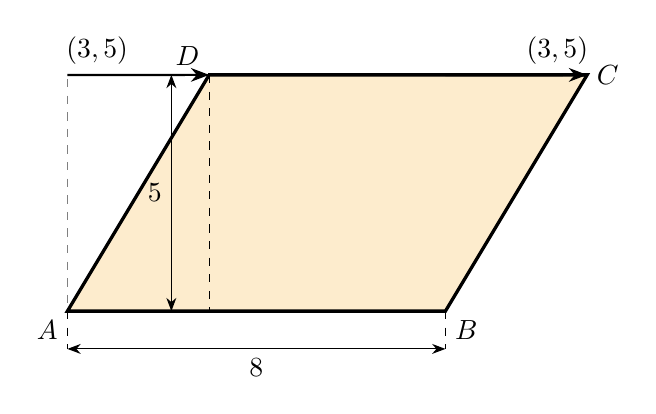
\begin{tikzpicture}[scale=0.6, >=Stealth]
  % persegi panjang asal (pudar)
  \draw[gray, dashed] (0,0) -- (8,0) -- (8,5) -- (0,5) -- cycle;

  % jajargenjang
  \coordinate (A) at (0,0);
  \coordinate (B) at (8,0);
  \coordinate (C) at (11,5);
  \coordinate (D) at (3,5);

  \fill[accent!25] (A) -- (B) -- (C) -- (D) -- cycle;
  \draw[very thick] (A) -- (B) -- (C) -- (D) -- cycle;

  % vektor pergeseran yang sama dipakai dua kali
  \draw[->, thick] (0,5) -- (D) node[midway, above left] {$(3,5)$};
  \draw[->, thick] (8,5) -- (C) node[midway, above right] {$(3,5)$};

  % label titik
  \node[below left] at (A) {$A$};
  \node[below right] at (B) {$B$};
  \node[right] at (C) {$C$};
  \node[above left] at (D) {$D$};

  % panjang alas
  \draw[<->] (0,-0.8) -- (8,-0.8) node[midway, below] {$8$};
  \draw[dashed] (0,0) -- (0,-0.8);
  \draw[dashed] (8,0) -- (8,-0.8);

  % tinggi
  \draw[dashed] (3,5) -- (3,0);
  \draw[<->] (2.2,0) -- (2.2,5) node[midway, left] {$5$};
\end{tikzpicture}
\end{center}

Kedua sisi miring digambar dari vektor yang sama $(3,5)$, sehingga sama panjang dan sejajar secara otomatis.

Luasnya tetap $L = 8 \times 5 = 40$, sama dengan persegi panjang asalnya.

\end{document}
